\section*{Mateusz Okoń}

Fragment tabeli 1 ligi polskiej (patrz Tabela \ref{tab:XD}).

\begin{table}[htbp]
    \centering
\begin{tabular}{llll}
Lp. & Drużyna       & M. & Pkt. \\
1   & Arka Gdynia   & 15 & 29   \\
2   & Odra Opole    & 15 & 27   \\
3   & Lechia Gdańsk & 15 & 26   \\
4   & Górnik Leczna & 15 & 26   \\
5   & GKS Tychy     & 15 & 25   \\
6   & Miedź Legnica & 15 & 24   \\
7   & Wisła Płock   & 15 & 23   \\
8   & Motor Lublin  & 15 & 23   \\
9   & Wisła Kraków  & 15 & 22   \\
10  & Bruk-Bet      & 15 & 20  
\end{tabular}
    \caption{Tabela 1 ligi}
    \label{tab:XD}
\end{table}


Trener jednego z zespołów 1 ligi polskiej (patrz Rysunek \ref{fig:gf}).
\begin{figure}[htbp]
    \centering
    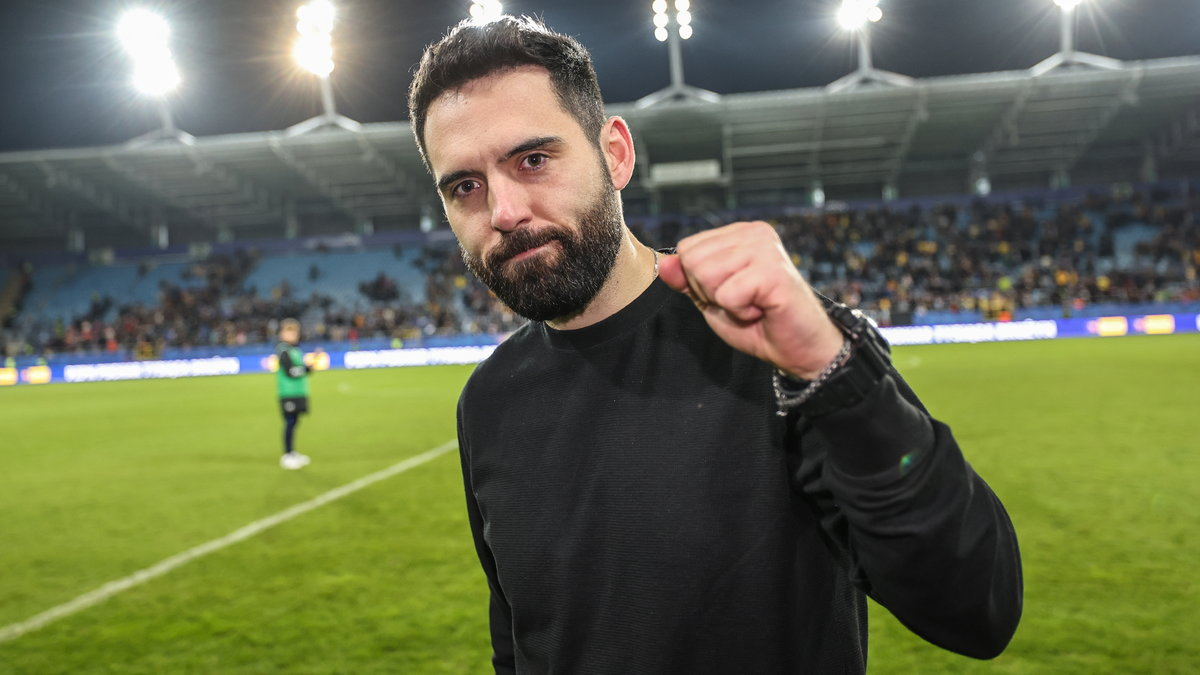
\includegraphics[width=0.8\textwidth, height=0.4\textwidth]{gf}
    \caption{Goncalo Feio}
    \label{fig:gf}    
\end{figure}

\section*{Wyrażenie matematyczne}
$sin^2x+cos^2x =1$ \\
$a^2+b^2= c^2$

\section*{Listy}
Lista 10 najbogatszych ludzi na świecie:
\begin{enumerate}
    \item Bernard Arnault (LVMH — 217,3 mld dol.)
    \item Elon Musk (Tesla, SpaceX, Twitter — 178,3 mld dol.)
    \item Jeff Bezos (Amazon — 126,3 mld dol.)
    \item Larry Ellison (Oracle — 111,9 mld dol.)
    \item Warren Buffett (Berkshire Hathaway — 108,5 mld dol.)
    \item Bill Gates (Microsoft, inwestycje — 104,5 mln dol.)
    \item Carlos Slim Helu (América Móvil — 91,7 mld dol.)
    \item Larry Page (Google — 85,8 mld dol.)
    \item Mukesh Ambani (Reliance Industries — 83,7 mld dol)
    \item Sergey Brin (Google — 82,2 mld dol.)
\end{enumerate}

Lista przykładowych owoców:
\begin{itemize}
    \item Jabłko
    \item Gruszka
    \item Śliwka
    \item Banan
    \item Ananas
    \item Cytryna
    \item Granat
    \item Arbuz
    \item Pomarańcza
    \item Malina
\end{itemize}

\section*{Przykładowy tekst wraz ze stylizacją}
\textbf{Sportem} są wszelkie formy \underline{aktywności fizycznej}\\
Dodatkowo \textbf{sport} wpływa na wypracowanie lub poprawienie kondycji \textit{fizycznej i psychicznej}.


